\section{Tasas de desarrollo y mortalidad}

Como se mencionó anteriormente en la sección \ref{sec:cap-3-cambio-climatico}, las tasas de desarrollo,
supervivencia de las distintas etapas del Aedes Aegypti, son susceptibles a los efectos de la
temperatura. En esta sección se presentan los resultados obtenidos, mediante el proceso el proceso
evolutivo, y pruebas realizadas para validar el desarrollo y la mortalidad de las distintas etapas del
Aedes Aegypti.



\subsection{Huevo}
Para el análisis de la tasa de desarrollo, en días, del huevo de Aedes aegypti, se incluyeron
los huevos que se desarrollaron completamente para pasar a ser una larva. Con el fin de realizar
una comparativa con los resultados obtenidos, en la \tabref{tab:desarrollo-huevo-test} se
utiliza como referencia los resultados obtenidos por \cite{BESERRA2006}, donde se presentan los
requerimientos térmicos para el desarrollo del aedes aegypti en condiciones naturales, para 5
cepas de Aedes Aegyti, provenientes de diferentes  poblaciones, a 5 temperaturas constantes
(18-34\textcelsius).


\begin{table}[H]
    \begin{minipage}{\textwidth}
        \caption{\label{tab:desarrollo-huevo-test} Análisis de la tasa de desarrollo, en días, de
        los huevos de Aedes aegypti a cinco temperaturas constantes (18-34 \textcelsius).}

        \begin{tabular}{p{5cm} c c c c c c }
            \hline \\
            Población    &18 \textcelsius & 22 \textcelsius & 26 \textcelsius & 30 \textcelsius & 34 \textcelsius & Media General\\

            \hline
            \hline \\
            Boqueirão            & 9,3 $^{b}$  & 6,5  & 3,9  & 3,3  & 3,5  & 4,3  \\
            B. dos Santos        & -- $^{a}$   & 5,9  & 4,3  & 3,7  & 2,9  & 4,2  \\
            C. Grande            & -- $^{a}$   & 5,5  & 3,4  & 4,4  & 3    & 4,07 \\
            Itaporanga           & 9,2 $^{b}$  & 6,2  & 4,7  & 3,1  & 3,5  & 4,38 \\
            Remígio              & -- $^{a}$   & 6    & 4,5  & 2    & 2,5  & 3.75 \\
            Media Predicha$^{c}$ & 6.61 $^{b}$ & 5,1  & 3.9  & 3.03 & 2.37 & 3.6  \\
            Media Obtenida$^{d}$ & 6.08 $^{b}$ & 5.06 & 3.03 & 3.03 & 2.02 & 3.29 \\

        \end{tabular}
        \footnotetext[1]{No hubo desarrollo embrionario a 18\textcelsius, \cite{BESERRA2006}.}
        \footnotetext[2]{Como no hubo desarrollo embrionario en las demas poblaciones a 18\textcelsius,
        se decidió no incluir estos datos en la media general, sólo representa el promedio para
        estas poblaciones \cite{BESERRA2006}.}
        \footnotetext[3]{Resultados obtenidos por el modelo de Sharpe \& DeMichele.}
        \footnotetext[4]{Resultados obtenidos mediante el proceso evolutivo.}
    \end{minipage}
\end{table}

En la \figref{fig:desarrollo-huevo-baserra2006}, se puede observar una compartiva con los
valores observados en \cite{BESERRA2006}, la media predicha y la media obtenida. En general se
obtuvo un desarrollo de $3.29$ días a 4 temperaturas constantes (22, 26, 30, 34 \textcelsius), con
una diferencia de, $0,97$, $0,87$, $0,87$, $1,15$ y $0,57$ días con la media general de los
valores observados en \cite{BESERRA2006} para las poblaciones de Boqueirão, B. dos Santos, C.
Grande, Itaporanga y Remígio respectivamente. Los autores de \cite{BESERRA2006}, señalan que a
18 \textcelsius, no existe desarrollo embrionario para las poblaciones de B. dos Santos, C. Grande
y Remígio, por lo que estos resultados no fueron incluidos en el calculo de la media general. En
relación a la media predicha, que fue obtenida mediante el modelo de \cite{sharpe1977reaction}, se
obtuvo una diferencia de $0,32$ días con la media obtenida.

\begin{figure}[H]
\begin{minipage}{\textwidth}
    \begin{tabular}{c c }
        \initbox
        \num\putindeepbox[7pt]{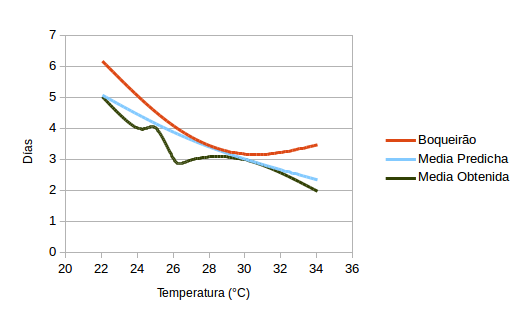
\includegraphics[width=0.4\textwidth]{capitulo-6/graphics/desarrollo-huevos-1.png}} &
        \num\putindeepbox[7pt]{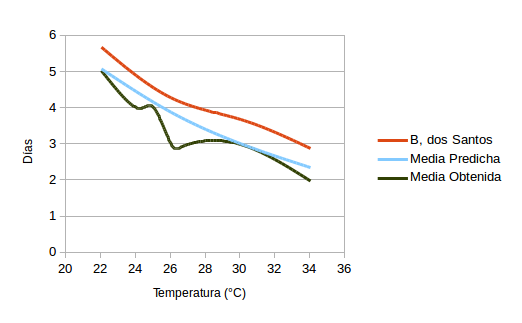
\includegraphics[width=0.4\textwidth]{capitulo-6/graphics/desarrollo-huevos-2.png}} \\

        \num\putindeepbox[7pt]{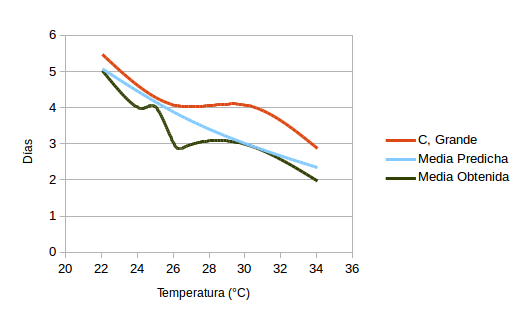
\includegraphics[width=0.4\textwidth]{capitulo-6/graphics/desarrollo-huevos-3.png}} &
        \num\putindeepbox[7pt]{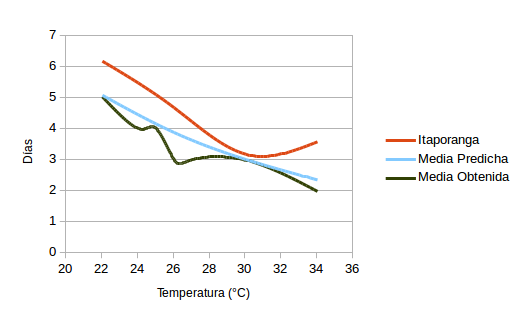
\includegraphics[width=0.4\textwidth]{capitulo-6/graphics/desarrollo-huevos-4.png}} \\

        \num\putindeepbox[7pt]{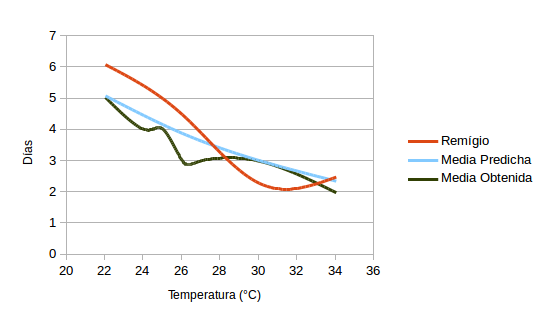
\includegraphics[width=0.4\textwidth]{capitulo-6/graphics/desarrollo-huevos-5.png}} &
        \num\putindeepbox[7pt]{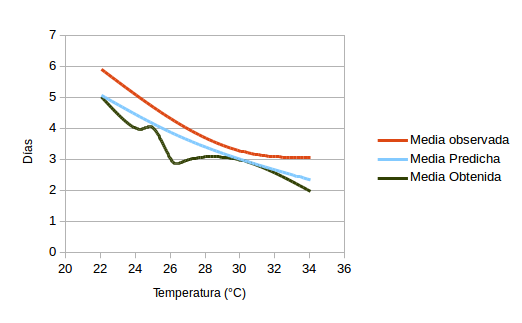
\includegraphics[width=0.4\textwidth]{capitulo-6/graphics/desarrollo-huevos-6.png}} \\
    \end{tabular}

    \caption{\label{fig:desarrollo-huevo-baserra2006}
    Comparativa entre ,la media obtenida, la media predicha y las medias observadas por \cite{
    BESERRA2006} en distintas pobalciones a 4 temperaturas contantes (18-34 \textcelsius) para
    las tasas de desarrollo de los huevos del Aedes Aegypti.}

    \footnotetext[1]{Tasa de desarrollo de Boqueirão en comparación con la media predicha y obtenida.}
    \footnotetext[2]{Tasa de desarrollo de B. dos Santos en comparación con la media predicha y obtenida.}
    \footnotetext[3]{Tasa de desarrollo de C. Grande en comparación con la media predicha y obtenida.}
    \footnotetext[4]{Tasa de desarrollo de Itaporanga en comparación con la media predicha y obtenida.}
    \footnotetext[5]{Tasa de desarrollo de Remígio en comparación con la media predicha y obtenida.}
    \footnotetext[6]{Media observada en los poblados de Boqueirão, B. dos Santos, C. Grande, Itaporanga, Remígio en comparación con la media predicha y obtenida.}

\end{minipage}
\end{figure}

%%Analisis de la Motalidad
En cuanto a la tasa de mortalidad diaria, \cite{otero2006stochastic} la define como una constante
independiente a la temperatura del 1\%, en la \tabref{tab:mortalidad-huevo-test} se presentan
los porcentajes de mortalidad obtenidos a 9 temperaturas constantes. En genral se obtuvo, un $1,64$
\% de mortalidad diaria, $98,36$ \% de supervivencia y un error del $0,64$ \% en comparación al 1
\% esperado.

\begin{table}[H]
    \centering
    \begin{minipage}{\textwidth}
        \caption{ \label{tab:mortalidad-huevo-test} Análisis de la tasa de mortalidad del huevo del
         Aedes Aegypti a nueve temperaturas constantes (18-34 \textcelsius).}

        \begin{tabular}{c c c c c c}
                    \hline \\
                    Temperatura&Huevos$^{a}$&Total$^{b}$&Mortalidad$^{c}$&Supervivencia$^{d}$\\
                    \textcelsius& Muertos   & de Huevos & (\%)           & (\%)\\
                    \hline
                    \hline \\
                    18            & 2618    & 156387   & 1,67 & 98,33\\
                    20            & 10962   & 659232   & 1,66 & 98,34\\
                    22            & 19089   & 1148391  & 1,66 & 98,34\\
                    24            & 53216   & 3228224  & 1,65 & 98,35\\
                    25            & 108324  & 6570126  & 1,65 & 98,35\\
                    26            & 126936  & 7753716  & 1,64 & 98,36\\
                    27            & 157990  & 9649119  & 1,64 & 98,36\\
                    30            & 611360  & 37347840 & 1,64 & 98,36\\
                    34            & 185972  & 11433440 & 1,63 & 98,37\\
                    Media General & 1276467 & 77946475 & 1,64 & 98,36\\
        \end{tabular}
        \footnotetext[1]{Total de huevos muertos en cada tempratura.}
        \footnotetext[2]{Total de huevos generados en cada temperatura}
        \footnotetext[3]{Tasa de mortalidad porcetual obtenida.}
        \footnotetext[4]{Tasa de supervivencia porcetual obtenida.}
    \end{minipage}
\end{table}

Los errores obtenidos se originan duarante el redondeo realizado al aplicar la tasa de
mortalidad diaria en cada colonia, debido a que el modelo, a la hora de calcular la cantidad de
huevos a ser eliminados de la colonia a la que pertenecen, solo permite eliminar a un número entero
de huevos. Si contamos con un grupo 10 de colonias cada una con 63 huevos, un total de 630 huevos.
Aplicando la tasa de mortalidad $0,01$ en cada colonia se obtine un total de $0,63$, aplicando el
operador de redondeo,definido por la ecuación \eqref{eq:operador-redondeo}, es $1$ huevo por
colonia. Al eliminar un huevo por colonia, en total se eliminarán 10 huevos en comparación al $6,3$
que se obtendría al eliminar $0,63$ huevos por colonia. En la tabla
\tabref{tab:mortalidad-huevo-error} se presentan los resultados del análisis realizado.

\begin{table}
    \begin{minipage}{\textwidth}
        \caption{ \label{tab:mortalidad-huevo-error} Análisis de la aplicación de la tasa de mortalidad entera del huevo del Aedes Aegypti.}

        \begin{tabular}{p{4cm} p{4cm} p{3cm} l }
                    \hline \\
                    Colonia & Cantidad de Huevos & Mortalidad$^{a}$ & Mortalidad Entera$^{b}$\\
                    \hline
                    \hline \\

                    1       & 63  & 0,63 & 1\\
                    2       & 63  & 0,63 & 1\\
                    3       & 63  & 0,63 & 1\\
                    4       & 63  & 0,63 & 1\\
                    5       & 63  & 0,63 & 1\\
                    6       & 63  & 0,63 & 1\\
                    7       & 63  & 0,63 & 1\\
                    8       & 63  & 0,63 & 1\\
                    9       & 63  & 0,63 & 1\\
                    10      & 63  & 0,63 & 1\\
                    Media General  & 630 & 6,3 & 10\\

        \end{tabular}
    \footnotetext[1]{Cantidad de huevos a eliminar al aplicar la de mortalidad de 0,01 definida en
    \cite{otero2006stochastic}.}
    \footnotetext[2]{Cantidad de huevos a eliminar aplicando el operador de redondeo definido por la ecuación \eqref{eq:operador-redondeo}.}
    \end{minipage}
\end{table}

\subsection{Desarrollo de las larvas}
Para el análisis de la tasa de desarrollo, en días, de las larvas, del Aedes aegypti, incluyeron
aquellas que culminaron su estado para pasar a ser una pupa. Existen diversos
estudios, que han reportado que tasa de desarrollo de las larvas, se encuentra influenciada por la
temperaturura y varia de acuerdo a las localidades y subespecies. A continuación se mencionaran
algunos estudios realizados correspondientes a la tasa de desarrollo en días de la larva, con el
fin de realizar una comparación con los resultados obtenidos.

En \cite{rueda1990temperature}, se reporta el efecto de  temperaturas constantes sobre las tasas
de desarrollo, el crecimiento y la supervivencia de los estados inmaduros de Aeedes aegypti,
determinadas en condiciones de laboratorio, y el modelo dependiente de la temperatura de
\cite{sharpe1977reaction}. En la tabla \ref{tab:desarrollo-larva-rueda1990temperature-test} se
presentan los resultados obtenidos a seis temperaturas constantes(15-34 \textcelsius) en
comparación a los obtenidos en \cite{rueda1990temperature}.

En la Figura \ref{fig:desarrollo-larva-rueda1990}, se puede observar una compartiva con los
valores observados en \cite{rueda1990temperature}, la media predicha y la media obtenida. En
general se obtuvo un desarrollo de $13,59$ días para 6 temperaturas contantes (15, 20, 25, 27,
30, 34 \textcelsius), con una diferencia de $-0,38$ y $-0,6$ días con la media general de los
valores observados en \cite{rueda1990temperature} para la media y la median observada respectivamente. En relación a la media predicha, que fue obtenida mediante el modelo de
\cite{sharpe1977reaction}, se obtuvo una diferencia de $-0,37$ días con la media otenida.

\begin{table}
    \begin{minipage}{\textwidth}
        \caption{ \label{tab:desarrollo-larva-rueda1990temperature-test} Análisis de la tasa de desarrollo de las larvas del Aedes Aegypti a seis temperaturas constantes
        (15-34 \textcelsius).}
        \begin{tabular}{p{5cm} c c c c c c c}
            \hline\\
            Resultados & 15\textcelsius & 20\textcelsius & 25\textcelsius & 27\textcelsius
            & 30\textcelsius & 34\textcelsius &  Media General\\
            \hline
            \hline \\
            Media Observada$^{a}$   & 46,83 & 9,31  & 8,61 & 4,47 & 4,99 & 5,06 & 13,21\\
            Mediana Observada$^{a}$ & 45,82 & 9,06  & 8,7  & 4,46 & 4,86 & 5,04 & 12,99\\
            Media Predicha$^{b}$    & 42,33 & 14,89 & 6,48 & 5,28 & 4,72 & 5,61 & 13,22\\
            Media obtenida$^{c}$    & 44,34 & 14,99 & 6,62 & 5,53 & 4,47 & 5,6 & 13,59\\

        \end{tabular}
        \footnotetext[1]{Valores observados por \cite{rueda1990temperature}.}
        \footnotetext[2]{Resultados obtenidos por el modelo de \cite{sharpe1977reaction}.}
        \footnotetext[3]{Resultados obtenidos mediante el proceso evolutivo.}
    \end{minipage}
\end{table}


\begin{figure}
    \centering
    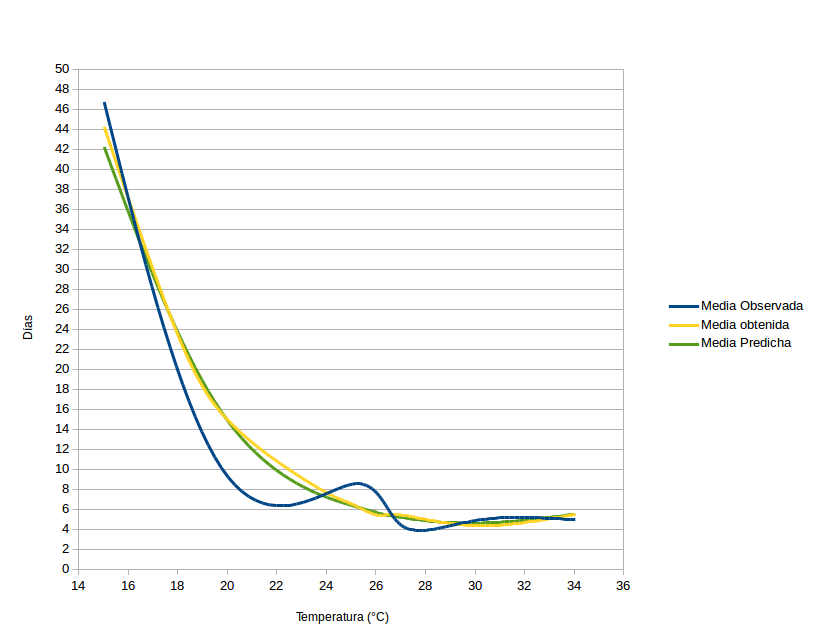
\includegraphics[width=1\textwidth]{capitulo-6/graphics/desarrollo-larva-rueda.png}
    \caption{\label{fig:desarrollo-larva-rueda1990}
    Comparativa entre ,la media obtenida, la media predicha y las media observada por \cite{
    rueda1990temperature} en distintas pobalciones a 6 temperaturas contantes (15-34 \textcelsius)
    para las tasas de desarrollo de las larvas del Aedes Aegypti.}
\end{figure}

%Comparación con los datos de BASERRA

En \cite{BESERRA2006}, se presentan los requerimientos térmicos para el desarrollo del aedes
aegypti en condiciones naturales, para 5 cepas de Aedes Aegyti, provenientes de diferentes
poblaciones, a 5 temperaturas constantes (18-34\textcelsius). En la tabla
\ref{tab:desarrollo-larva-baserra2006-test} se presentan los resultados obtenidos a cinco
temperaturas constantes(15-34 \textcelsius) en comparación a las tasas de desarrollo obtenidas en
\cite{BESERRA2006} para las larvas del Aedes Aegypti.

En la Figura \ref{fig:desarrollo-larva-baserra2006}, se puede observar una compartiva con los
valores observados en \cite{BESERRA2006}, la media predicha y la media obtenida. En general se
obtuvo un desarrollo de $9,96$ días para 5 temperaturas contantes (18, 22, 26, 30, 34
\textcelsius), con una diferencia de $1,04$, $1,64$, $-0,36$, $1,24$ y $0,94$ días con la media
general de los valores observados en \cite{BESERRA2006} para las poblaciones de Boqueirão, B. dos
Santos, C. Grande, Itaporanga y Remígio respectivamente. En relación a la media predicha, que fue
obtenida mediante el modelo de \cite{sharpe1977reaction}, se obtuvo una diferencia de $-0,22$ días
con la media obtenida.

\begin{table}
    \begin{minipage}{\textwidth}
        \caption{\label{tab:desarrollo-larva-baserra2006-test} Análisis de la tasa de desarrollo de
        las larvas del Aedes Aegypti a cinco temperaturas constantes (15-34 \textcelsius).}
        \begin{tabular}{p{5cm} c c c c c c }
            \hline\\
            Población    &18 \textcelsius & 22 \textcelsius & 26 \textcelsius & 30 \textcelsius
            & 34 \textcelsius & Media General\\
            \hline
            \hline \\
            Boqueirão$^{a}$        & 19,6  & 13,4  & 8,7  & 6,4  & 6,9 & 11\\
            B, dos Santos$^{a}$    & 18,9  & 13,4  & 10,2 & 7,9  & 7,5 & 11,6\\
            C, Grande$^{a}$        & 18,3  & 11,1  & 6,6  & 5,8  & 6   & 9,6\\
            Itaporanga$^{a}$       & 21    & 12,3  & 7,3  & 5,9  & 9,7 & 11,2\\
            Remígio$^{a}$          & 18,9  & 15,8  & 8,4  & 5,4  & 6   & 10,9\\
            Media obtenida$^{b}$   & 23,37 & 10,85 & 5,51 & 4,47 & 5,6 & 9,96\\
        \end{tabular}
        \footnotetext[1]{Los valores presentados para estas poblaciones fueron tomados de
         \cite{BESERRA2006}.}
        \footnotetext[2]{Resultados obtenidos mediante el proceso evolutivo.}
    \end{minipage}
\end{table}


\begin{figure}
\begin{minipage}{\textwidth}
    \begin{tabular}{c c }
        \initbox
        \num\putindeepbox[7pt]{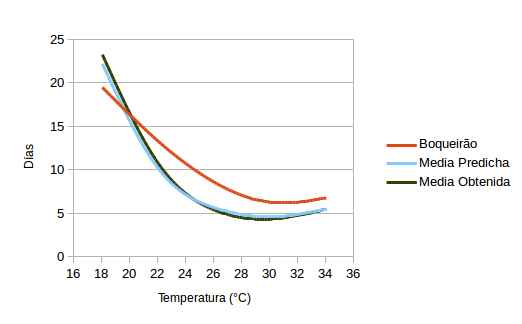
\includegraphics[width=0.4\textwidth]{capitulo-6/graphics/desarrollo-larva-1.png}} &
        \num\putindeepbox[7pt]{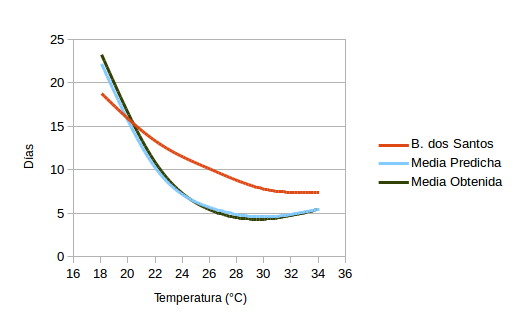
\includegraphics[width=0.4\textwidth]{capitulo-6/graphics/desarrollo-larva-2.png}} \\

        \num\putindeepbox[7pt]{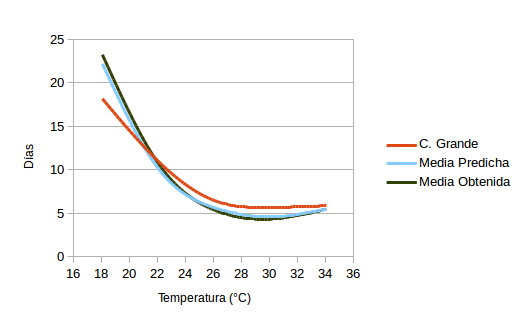
\includegraphics[width=0.4\textwidth]{capitulo-6/graphics/desarrollo-larva-3.png}} &
        \num\putindeepbox[7pt]{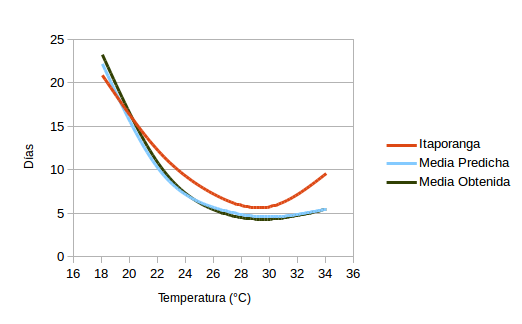
\includegraphics[width=0.4\textwidth]{capitulo-6/graphics/desarrollo-larva-4.png}} \\

        \num\putindeepbox[7pt]{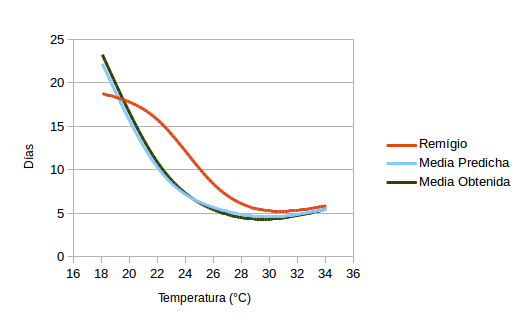
\includegraphics[width=0.4\textwidth]{capitulo-6/graphics/desarrollo-larva-5.png}} &
        \num\putindeepbox[7pt]{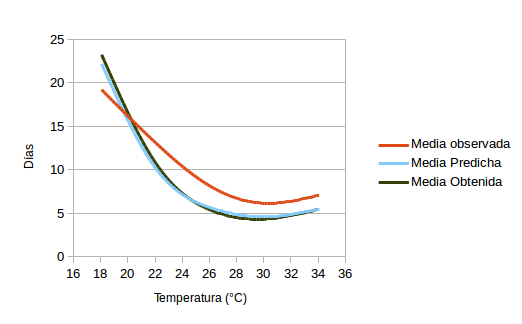
\includegraphics[width=0.4\textwidth]{capitulo-6/graphics/desarrollo-larva-6.png}} \\
    \end{tabular}

    \caption{\label{fig:desarrollo-larva-baserra2006}
    Comparativa entre ,la media obtenida, la media predicha y las medias observadas por \cite{
    BESERRA2006} en distintas pobalciones a 4 temperaturas contantes (18-34 \textcelsius) para
    las tasas de desarrollo de las larvas del Aedes Aegypti.}

    \footnotetext[1]{Tasa de desarrollo de Boqueirão en comparación con la media predicha y obtenida.}
    \footnotetext[2]{Tasa de desarrollo de B. dos Santos en comparación con la media predicha y obtenida.}
    \footnotetext[3]{Tasa de desarrollo de C. Grande en comparación con la media predicha y obtenida.}
    \footnotetext[4]{Tasa de desarrollo de Itaporanga en comparación con la media predicha y obtenida.}
    \footnotetext[5]{Tasa de desarrollo de Remígio en comparación con la media predicha y obtenida.}
    \footnotetext[6]{Media observada en los poblados de Boqueirão, B. dos Santos, C. Grande, Itaporanga, Remígio en comparación con la media predicha y obtenida.}

\end{minipage}
\end{figure}

\subsection{Pupa}
Para el análisis de la tasa de desarrollo, en días, de las pupas, del Aedes aegypti, incluyeron
las pupas que se desarrollaron completamente para pasar a ser un adulto. Existen diversos
estudios, que han reportado que tasa de desarrollo de las pupas, se encuentra influenciada por la
temperaturura y varia de acuerdo a las localidades y subespecies. A continuación se mencionaran
algunos estudios realizados correspondientes a la tasa de desarrollo en días de la pupa, con el
fin de realizar una comparación con los resultados obtenidos.

En \cite{rueda1990temperature}, se reporta el efecto de temperaturas constantes sobre las tasas
de desarrollo, el crecimiento y la supervivencia de los estados inmaduros de Aeedes aegypti,
determinadas en condiciones de laboratorio, y el modelo dependiente de la temperatura de
\cite{sharpe1977reaction}. En la \tabref{tab:desarrollo-pupa-rueda1990temperature-test} se
presentan los resultados obtenidos a seis temperaturas constantes(15-34 \textcelsius) en
comparación a los obtenidos en \cite{rueda1990temperature}.

En la \figref{fig:desarrollo-pupa-rueda1990}, se puede observar una compartiva con los
valores observados en \cite{rueda1990temperature}, la media predicha y la media obtenida. En
general se obtuvo un desarrollo de $2,83$ días para 6 temperaturas contantes (15, 20, 25, 27,
30, 34 \textcelsius), con una diferencia de $0,39$ y $0,36$ días con la media general de los
valores observados en \cite{rueda1990temperature} para la media y la median observada respectivamente. En relación a la media predicha, que fue obtenida mediante el modelo de
\cite{sharpe1977reaction}, se obtuvo una diferencia de $0,2$ días con la media obtenida.


\begin{table}
    \begin{minipage}{\textwidth}
        \caption{ \label{tab:desarrollo-pupa-rueda1990temperature-test} Análisis de la tasa de desarrollo de las pupas del Aedes Aegypti a seis temperaturas constantes
        (15-34 \textcelsius).}
        \begin{tabular}{p{5cm} c c c c c c c}
            \hline\\
            Resultados & 15\textcelsius & 20\textcelsius & 25\textcelsius & 27\textcelsius
            & 30\textcelsius & 34\textcelsius &  Media General\\
            \hline
            \hline \\
            Media Observada$^{a}$   & 8,49 & 3,11 & 3,03 & 1,79 & 1,82 & 1,09 & 3,22\\
            Mediana Observada$^{a}$ & 8,46 & 3,04 & 2,98 & 1,81 & 1,79 & 1,05 & 3,19\\
            Media Predicha$^{b}$    & 6,9  & 4,1  & 2,5  & 2,06 & 1,56 & 1,08 & 3,03\\
            Media obtenida$^{c}$    & 6,14 & 4,26 & 2,17 & 2,17 & 1,11 & 1,14 & 2,83\\
        \end{tabular}
        \footnotetext[1]{Valores observados por \cite{rueda1990temperature}.}
        \footnotetext[2]{Resultados obtenidos por el modelo de \cite{sharpe1977reaction}.}
        \footnotetext[3]{Resultados obtenidos mediante el proceso evolutivo.}
    \end{minipage}
\end{table}

\begin{figure}
    \centering
    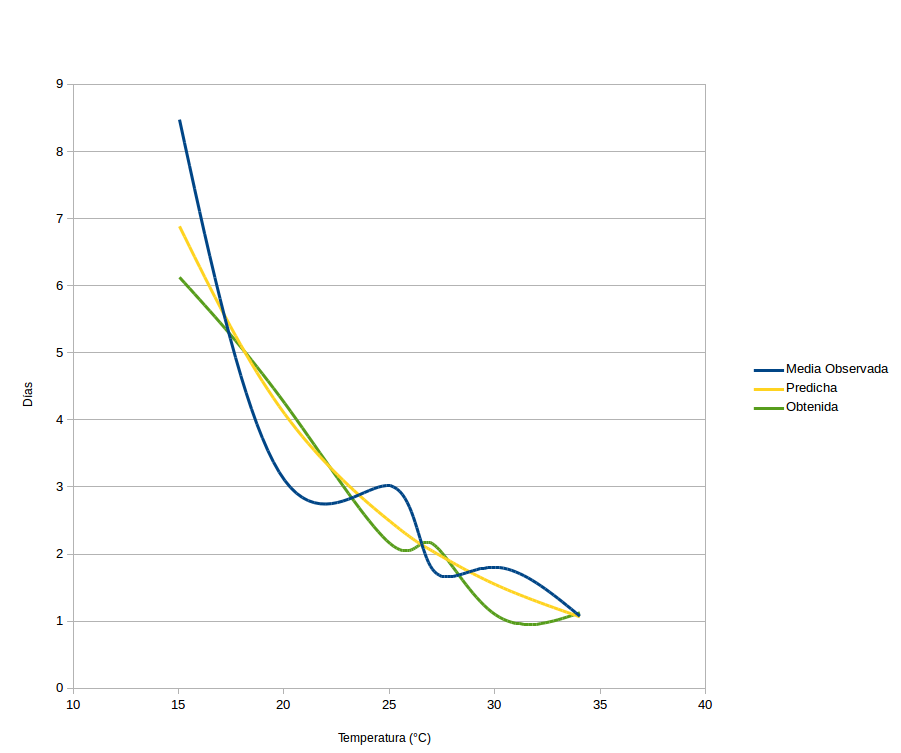
\includegraphics[width=1\textwidth]{capitulo-6/graphics/desarrollo-pupa-rueda.png}
    \caption{\label{fig:desarrollo-pupa-rueda1990}
    Comparativa entre ,la media obtenida, la media predicha y las media observada por \cite{
    rueda1990temperature} en distintas pobalciones a 6 temperaturas contantes (15-34 \textcelsius)
    para las tasas de desarrollo de las pupas del Aedes Aegypti.}

\end{figure}


En \cite{BESERRA2006}, se presentan los requerimientos térmicos para el desarrollo del aedes
aegypti en condiciones naturales, para 5 cepas de Aedes Aegyti, provenientes de diferentes
poblaciones, a 5 temperaturas constantes (18-34\textcelsius). En la
\tabref{tab:desarrollo-pupa-baserra2006-test} se presentan los resultados obtenidos a cinco
temperaturas constantes(15-34 \textcelsius) en comparación a las tasas de desarrollo obtenidas en
\cite{BESERRA2006} para las pupas del Aedes Aegypti.

En la \figref{fig:desarrollo-pupa-baserra2006}, se puede observar una compartiva con los
valores observados en \cite{BESERRA2006}, la media predicha y la media obtenida. En general se
obtuvo un desarrollo de $2,57$ días para 5 temperaturas contantes (18, 22, 26, 30, 34
\textcelsius), con una diferencia de $0,57$, $0,43$, $0,43$, $0,41$ y $0,25$ días con la media
general de los valores observados en \cite{BESERRA2006} para las poblaciones de Boqueirão, B. dos
Santos, C. Grande, Itaporanga y Remígio respectivamente. En relación a la media predicha, que fue
obtenida mediante el modelo de \cite{sharpe1977reaction}, se obtuvo una diferencia de $0,09$ días
con la media obtenida.

\begin{table}
    \begin{minipage}{\textwidth}
        \caption{\label{tab:desarrollo-pupa-baserra2006-test} Análisis de la tasa de desarrollo de
        las pupas del Aedes Aegypti a cinco temperaturas constantes (15-34 \textcelsius).}
        \begin{tabular}{p{5cm} c c c c c c }
            \hline\\
            Población    &18 \textcelsius & 22 \textcelsius & 26 \textcelsius & 30 \textcelsius
            & 34 \textcelsius & Media General\\
            \hline
            \hline \\
            Boqueirão$^{a}$      & 7,2  & 3,2  & 2,7  & 1,2  & 1,4  & 3,14\\
            B, dos Santos$^{a}$  & 6,4  & 3,2  & 2,1  & 2,1  & 1,2  & 3\\
            C, Grande$^{a}$      & 6,7  & 2,7  & 2,4  & 1,6  & 1,6  & 3\\
            Itaporanga$^{a}$     & 6,6  & 3,2  & 2,3  & 1,4  & 1,4  & 2,98\\
            Remígio$^{a}$        & 6,3  & 3,3  & 2,3  & 1,1  & 1,1  & 2,82\\
            Media obtenida$^{c}$ & 5,24 & 3,21 & 2,17 & 1,11 & 1,14 & 2,57\\
        \end{tabular}
        \footnotetext[1]{Los valores presentados para estas poblaciones fueron tomados de
         \cite{BESERRA2006}.}
        \footnotetext[2]{Resultados obtenidos mediante el proceso evolutivo.}
    \end{minipage}
\end{table}



\begin{figure}
\begin{minipage}{\textwidth}
    \begin{tabular}{c c }
        \initbox
        \num\putindeepbox[7pt]{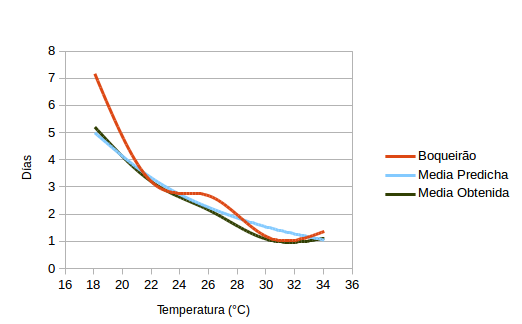
\includegraphics[width=0.4\textwidth]{capitulo-6/graphics/desarrollo-pupa-1.png}} &
        \num\putindeepbox[7pt]{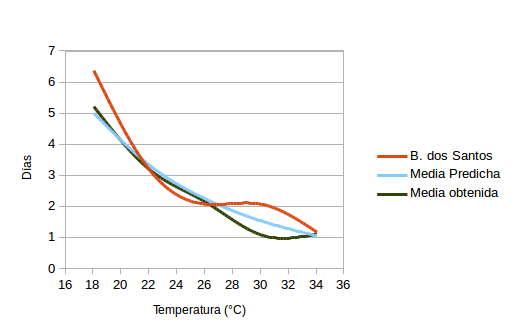
\includegraphics[width=0.4\textwidth]{capitulo-6/graphics/desarrollo-pupa-2.png}} \\

        \num\putindeepbox[7pt]{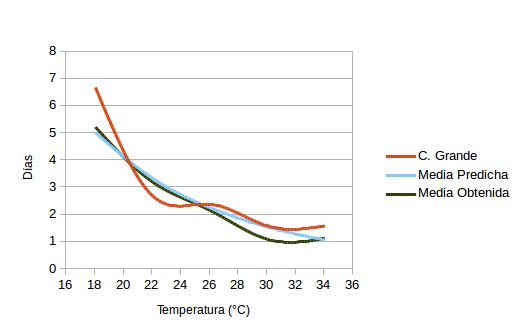
\includegraphics[width=0.4\textwidth]{capitulo-6/graphics/desarrollo-pupa-3.png}} &
        \num\putindeepbox[7pt]{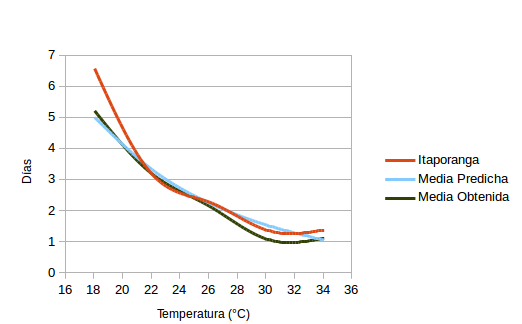
\includegraphics[width=0.4\textwidth]{capitulo-6/graphics/desarrollo-pupa-4.png}} \\

        \num\putindeepbox[7pt]{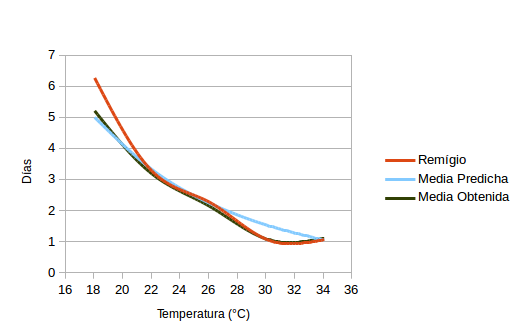
\includegraphics[width=0.4\textwidth]{capitulo-6/graphics/desarrollo-pupa-5.png}} &
        \num\putindeepbox[7pt]{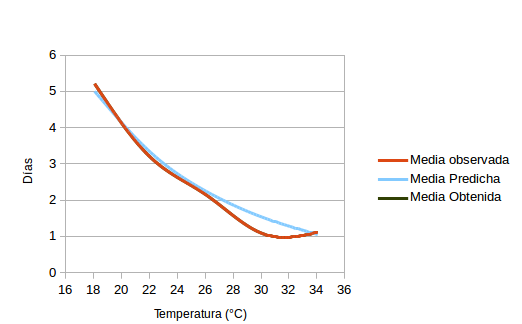
\includegraphics[width=0.4\textwidth]{capitulo-6/graphics/desarrollo-pupa-6.png}} \\
    \end{tabular}

    \caption{\label{fig:desarrollo-pupa-baserra2006}
    Comparativa entre ,la media obtenida, la media predicha y las medias observadas por \cite{
    BESERRA2006} en distintas pobalciones a 4 temperaturas contantes (18-34 \textcelsius) para
    las tasas de desarrollo de las pupas del Aedes Aegypti.}

    \footnotetext[1]{Tasa de desarrollo de Boqueirão en comparación con la media predicha y obtenida.}
    \footnotetext[2]{Tasa de desarrollo de B. dos Santos en comparación con la media predicha y obtenida.}
    \footnotetext[3]{Tasa de desarrollo de C. Grande en comparación con la media predicha y obtenida.}
    \footnotetext[4]{Tasa de desarrollo de Itaporanga en comparación con la media predicha y obtenida.}
    \footnotetext[5]{Tasa de desarrollo de Remígio en comparación con la media predicha y obtenida.}
    \footnotetext[6]{Media observada en los poblados de Boqueirão, B. dos Santos, C. Grande, Itaporanga, Remígio en comparación con la media predicha y obtenida.}

\end{minipage}
\end{figure}

\subsection{Adulto}
Como se menciona en la \secref{subsec:mortalidad} la tasa de la mortalidad utilizada fue
la definida en \cite{otero2006stochastic}, como una constante de valor 0.09 independiente de la
temperatura. En la \tabref{tab:mortalidad-diaria-adulto-test} se presentan los resultados
obtenidos de la tasa de mortalidad del Aedes aegypti a diez temperaturas constantes (18-34
\textcelsius). En general se  se obtuvo una mortalidad, diaria de $11,08$\% en comparación al 9\%
definido en \cite{otero2006stochastic} y el 10\% señalado en \cite{ThironIzcazaJ2003}.

\begin{table}[H]
    \caption{ \label{tab:mortalidad-diaria-adulto-test} Análisis de la tasa de mortalidad del adulto del Aedes aegypti a diez temperaturas constantes (15-34 \textcelsius).}
        \begin{tabular}{p{3cm} c c c }
                    \hline \\
                    Temperatura & Adultos Muertos & Total de Adultos & \% Mortalidad\\
                    \hline
                    \hline \\

                    15 \textcelsius & 270    & 2216    & 12,18\\
                    18 \textcelsius & 7099   & 68092   & 10,43\\
                    20 \textcelsius & 11050  & 99858   & 11,07\\
                    22 \textcelsius & 14250  & 117775  & 12,1\\
                    24 \textcelsius & 17708  & 157624  & 11,23\\
                    25 \textcelsius & 19500  & 175071  & 11,14\\
                    26 \textcelsius & 30804  & 268608  & 11,47\\
                    27 \textcelsius & 30957  & 278450  & 11,12\\
                    30 \textcelsius & 221381 & 2033769 & 10,89\\
                    34 \textcelsius & 27716  & 235984  & 11,74\\
                    Total           & 380735 & 3437447 & 11,08\\

        \end{tabular}
\end{table}

Los autores de \cite{ThironIzcazaJ2003} señalan que la mortalidad de una población de adultos, se encuentra entre el 50\% a los 7 días y un 95\% a los 30 días. En la
\tabref{tab:mortalidad-periodo-adulto-test} se presenta los resultados correspondientes a la mortalidad de los adultos a 7 y 30 días. En general se obtuvo un $54,96$\% a los 7 días y un
$96,66$\% a los 30 días, en comparación al 50\% y el 95\% señalados por señalado por los autores
de \cite{ThironIzcazaJ2003}.


\begin{table}[H]
    \centering
        \caption{ \label{tab:mortalidad-periodo-adulto-test} Análisis de la tasa de mortalidad del
        adulto del Aedes aegypti a nueve temperaturas constantes (15-34 \textcelsius) para los
        periodos de 7 y 30 días.}

        \begin{tabular}{p{3cm} c c c c c }
                    \hline \\
                    Temperatura & Total de & Muertos a  & Muertos a   & Mortalidad & Mortalidad\\
                    Temperatura & adultos  & los 7 días & los 30 días & 7 días(\%) & 30 días(\%)\\
                    \hline
                    \hline \\
                    18\textcelsius &370  & 177 & 305 & 56,08 & 82,43\\
                    20\textcelsius &526  & 295 & 508 & 57,89 & 96,58\\
                    22\textcelsius &672  & 389 & 659 & 54,03 & 98,07\\
                    24\textcelsius &818  & 442 & 797 & 54,55 & 97,43\\
                    25\textcelsius &869  & 474 & 846 & 54,67 & 97,35\\
                    26\textcelsius &900  & 492 & 878 & 55,1 & 97,56\\
                    27\textcelsius &882  & 486 & 861 & 54,99 & 97,62\\
                    30\textcelsius &991  & 545 & 962 & 56,72 & 97,07\\
                    34\textcelsius &744  & 422 & 730 & 56,72 & 98,12\\
                    Media general   & 6772 & 3722 & 6546 & 54,96 & 96,66\\

        \end{tabular}
\end{table}

Los errores obtenidos se originan durante el redondeo realizado al aplicar la tasa de
mortalidad diaria en cada colonia, debido a que el modelo, a la hora de calcular la cantidad de
adultos a ser eliminados de la colonia a la que pertenecen, solo permite eliminar a un número
entero de adultos. Si contamos con un grupo 10 de colonias cada una con 6 adultos cada una,
tenemos un total de 60 adultos.Aplicando la tasa de mortalidad $0,09$ en cada colonia se obtiene un
total de $0,54$, aplicando el operador de redondeo, definido por la ecuación
\eqref{eq:operador-redondeo}, es de $1$ adulto por colonia. Al eliminar un adulto por colonia, en
total se eliminarán 10 adultos en comparación al $5,4$ que se obtendría al eliminar $0,54$ adultos
por colonia. En la \tabref{tab:mortalidad-adulto-error} se presentan los resultados del
análisis realizado.

\begin{table}[H]
    \begin{minipage}{\textwidth}
        \caption{ \label{tab:mortalidad-adulto-error} Análisis de la aplicación de la tasa de
        mortalidad entera del adulto del Aedes Aegypti.}
        \begin{tabular}{p{3cm} c c c }
                    \hline \\
                    Colonia & Cantidad de Adultos & Mortalidad$^{a}$ & Mortalidad Entera$^{b}$\\
                    \hline
                    \hline \\
                    1       & 6  & 0,54 & 1\\
                    2       & 6  & 0,54 & 1\\
                    3       & 6  & 0,54 & 1\\
                    4       & 6  & 0,54 & 1\\
                    5       & 6  & 0,54 & 1\\
                    6       & 6  & 0,54 & 1\\
                    7       & 6  & 0,54 & 1\\
                    8       & 6  & 0,54 & 1\\
                    9       & 6  & 0,54 & 1\\
                    10      & 6  & 0,54 & 1\\
                    Total   & 60 & 5,4  & 10\\
        \end{tabular}
        \footnotetext[1]{Cantidad de adultos a eliminar al aplicar la de mortalidad de 0,09 definida en \cite{otero2006stochastic}.}
        \footnotetext[2]{Cantidad de adultos a eliminar aplicando el operador de redondeo definido por la ecuación \eqref{eq:operador-redondeo}.}
    \end{minipage}
\end{table}

